\documentclass[11.5pt,twocolumn]{article}
\setlength{\columnsep}{1cm}

%! ROOT=adventure.tex
\usepackage{array}
\usepackage{url}
\usepackage{dirtytalk}
\usepackage{graphicx}
\usepackage{lmodern}
\usepackage{mdframed}
\usepackage{xcolor}
\usepackage{xspace}

\newcommand\bodhran{Bodhr\'{a}n\xspace}
\newcommand{\pngname}[1]{\underline{\textit{\textsc{#1}}}}
\newcommand{\npcname}[1]{\underline{\textit{\textsc{#1}}}}
\newcommand{\tiro}[2]{tiro \textbf{#1} a difficolt\`{a} \textbf{#2}}

\newmdenv[linecolor=red,backgroundcolor=yellow!25]{infobox}
\newmdenv[linecolor=red,backgroundcolor=cyan!15]{dreambox}
\newmdenv[linecolor=red,backgroundcolor=red!15]{monsterbox}

\newcommand{\dvstat}[5]{
\textbf{DV}: #1 \\
\emph{1 DV}: #2 \\
\emph{2 DV}: #3 \\
\emph{3 DV}: #4 \\
\emph{Punti Vita}: #5 \\
}

\newcommand{\equip}[2]{
\emph{Armi}: #1 \\
\emph{Armatura}: #2 \\
}

\newcommand{\specialstat}[2]{
\emph{Abilit\`{a} Speciali}: #1 \\
\emph{Poteri Magici}: #2 \\
}

\newcommand{\npc}[2]{
\begin{infobox}
\begin{center}
\npcname{#1}
\end{center}
#2
\end{infobox}
}

\newcommand{\monster}[2]{
\begin{figure}[tb]
\begin{monsterbox}
\begin{center}
\npcname{#1}
\end{center}
#2
\end{monsterbox}
\end{figure}
}

\newcommand{\dream}[2]{
\begin{figure}[tb]
\begin{dreambox}
\begin{center}
\textbf{SOGNO:\\
\underline{#1}
}
\end{center}
#2
\end{dreambox}
\end{figure}
}

\newcommand{\object}[2]{
\begin{figure}[tb]
\begin{infobox}
\begin{center}
\textsc{#1}
\end{center}
#2
\end{infobox}
\end{figure}
}



\newcommand\politico{Ovius Silvius Quintilianus Emeritus}
\newcommand\duumvirouno{Publius Duronious Verax}
\newcommand\duumvirodue{Sextus Cornelius Bassianus Gallicus}
\newcommand\silvano{Silvanus Orontius Cremonensis}
\newcommand\balordi{Fratellanza della Morte}
\newcommand\prostitute{Prostitute di Mediolanum}
\newcommand\ninnananna{Ninna Nanna del Forestiero}
\newcommand\druidolepronti{Divinatrix Lepontious}
\newcommand\guerrieronemico{Guerrieri dei Corieltauvi}
\newcommand\predatore{Aquile}
\newcommand\canzone{Canzone dell'Oblio}
\newcommand\villico{Lucius Tubero Verbanicus}
\newcommand\ecatina{Naevia Seppiena Rutilia}
\newcommand\custosmorta{Lemonia Columella}
\newcommand\tarantasio{Tarantasium Adirato}
\newcommand\aquitani{Guerrieri Scelti Aquitani}
\newcommand\druidoaquitano{Druido Aquitano}
\newcommand\druidonemico{Mynio mab Gwawl}
\newcommand\cerchioceltico{Cerchio Celtico}
\newcommand\caponemico{Einion Owain}
\newcommand\confratelli{Il Ritorno del Fratello} %dream
\newcommand\amuletonero{Amuleto delle Fiamme Nere}

\begin{document}

\title{Il Quinto Confratello -- Una Avventura di Lex Arcana}
%\title{Trantasium -- Una Avventura di Lex Arcana}

\author{Stefano Cherubin}
\date{}

\maketitle

%%%%%%%%%%%%%%%%%%%%%%%%%%%%%%%%%%%%%%%%%%%%%%%%%%%%%%%%%%%%%%%%%%%%%%%%%%%%%%%
\lapart{Introduzione}
\lasection{Introduzione per i Giocatori}
Un messo imperiale vi riceve per conto del magister della Coorte Auxiliaria Arcana di Roma Urbe e vi conduce da uno scriba alle dipendenze del magister.
Entrambi sembrano molto rilassati, vi mostrano rispetto ma non sono intimoriti.
Vi spiegano che il magister ha richiesto la presenza di un piccolo contubernium per una ``missione formativa''.

Vi spiegano che sono ormai anni che la Coorte Auxiliaria Arcana opera nelle diverse province imperiali, scopre realt\`{a} inquietanti e protegge l'impero da pericoli nascosti e sconosciuti alla maggior parte della popolazione.
Nell'ultimo anno, diversi contubernia hanno svolto operazioni significative nelle varie zone montuose della Gallia Cisalpina; i loro rapporti sono stati archiviati -- come da protocollo -- negli archivi della sede della Corte Auxiliaria Arcana di Augusta Taurinorum.
Questa sede ha appena mandato -- nell'ambito di un regolare programma di aggiornamento -- alla sede di Roma Urbe una copia dei rapporti per informazione e per archivio.
Lo scriba fa una smorfia per farvi intendere che tutti queste operazioni sono molto importanti per l'impero ma soprattutto sono un carico di lavoro infinito per lui.

Lo scriba poi continua: \emph{%
Voi siete incaricati di andare da Roma verso Augusta Taurinorum per consegnare alla sede locale un fascicolo contenente un estratto degli aggiornamenti arrivati da diverse altre province imperiali.
Durante il viaggio potete leggervi qualche rapporto per imparare qualcosa di nuovo, se volete.
Tuttavia, non si tratta dell'unico motivo per cui inviamo un contubernium invece di un semplice messo.
Augusta Taurinorum pare non abbia pi\`{u} notizie di una custos (\custosmorta) inviata alla citt\`{a} di Mediolanum circa sei mesi fa.
Chiedono se Roma Urbe abbia ricevuto rapporti che la menzionino ma non ce ne sono.
Da Augusta Taurinorum non vi \`{e} menzione della missione a cui fu assegnata, ma questi rapporti sono spesso carenti di dettagli burocratici.
Cercate di capire cosa le sia successo.
Probabilmente non \`{e} nulla di grave, ma \custosmorta non ci sembra il tipo da sparire senza dare notizie.
Fate pure con calma, questi documenti dovevano essere ad Augusta Taurinorum un anno fa, un giorno o due in pi\`{u} non faranno certo la differenza.
}

%%%%%%%%%%%%%%%%%%%%%%%%%%%%%%%%%%%%%%%%%%%%%%%%%%%%%%%%%%%%%%%%%%%%%%%%%%%%%%%
\lasection{Introduzione per il Demiurgo}
%
Mediolanum \`{e} una citt\`{a} che riceve acqua da diversi fontanili, torrenti e fiumi.
A Mediolanum si iniziano ad avvertire i primi sintomi degli squilibri di ecosistemi pi\`{u} a monte.
I laghi alpini raccolgono abbondanti quantit\`{a} di acqua dolce e creano microclimi inusuali sulle loro sponde, oasi di terreno fertile e abbondanti riserve di pesca.
%delle vere e proprie gemme nascoste tra le alpi.
I laghi alpini meglio connessi ospitano anche residenze estive per facoltosi mercanti e politici locali.
Forse uno di loro ha allertato la coorte arcana, che ha inizialmente sottovalutato l'entit\`{a} dei pericoli che possono nascondersi anche nel pi\`{u} piccolo degli stagni.

I custodes sono inizialmente chiamati a fare dei semplici passacarte.
Questa \`{e} una opportunit\`{a} per il demiurgo di introdurre elementi narrativi o riferimenti a precedenti avventure in cui uno o pi\`{u} custodes del contubernium non fossero presenti.
Si consiglia di introdurre ai custodes l'esistenza del reame fatato e dei luoghi sottili come presentati dal manuale Britannia.~\cite{britannia_en}

Un luogo sottile \`{e} apparso sulle alpi e i custodes si ritroveranno ad esplorare i laghi alpini e scovare misteri nascosti tra le loro sponde e tra i loro flutti.
Un manipolo di celti provenienti da una dimenticata trib\`{u} britannica si appella all'alleanza del cerchio celtico e pianifica una ribellione contro Roma.
Un grosso predatore alieno a queste terre \`{e} comparso dal nulla,
%riemerso dal reame fatato dopo un viaggio durato chiss\`{a} quanti secoli,
e i custodes sono chiamati a ristabilire un equilibrio sostenibile nella regione.

%%%%%%%%%%%%%%%%%%%%%%%%%%%%%%%%%%%%%%%%%%%%%%%%%%%%%%%%%%%%%%%%%%%%%%%%%%%%%%%
\lasection{Sinossi}
\lasubsection{Parte I -- Passacarte}
%
Convocati a Roma, i custodes sono incaricati di andare ad Augusta Turinorum a consegnare documenti di archivio e di aggiornamento.
I custodes ricevono poche indicazioni e sono indirizzati a Mediolanum.
In questa fase i custodes possono raccogliere informazioni su missioni precedenti compiute da altri contubernia.

\lasubsection{Parte II -- Acque Irritate}
%
A Milano si avvertono flebili segni di squilibrio nella fauna acquatica del Verbanus e del Ticinus tuttavia nessuno sembra essersi reso conto di cosa sta accadendo.
Una ninfa che ha migrato lungo le acque del ticino fatica ad ambientarsi in luoghi pi\`{u} caldi e angusti dei laghi a cui era abituata prima.

\lasubsection{Parte III -- Il Predatore del Lago}
%
L'attenzione del contubernium si sposta verso il Verbannus.
Qui i custodes rilevano squilibri maggiori.
Con pazienza e astuzia, si pu\`{o} risalire il Tocis -- e lo Strona -- fino al Cusius Lacus dove un manipolo di celti ha attraversato un luogo sottile portando con s\`{e} con un drago dalla Britannia Secunda.
Il drago sembra tuttavia non essere intenzionato ad obbedirgli...

%%%%%%%%%%%%%%%%%%%%%%%%%%%%%%%%%%%%%%%%%%%%%%%%%%%%%%%%%%%%%%%%%%%%%%%%%%%%%%%
\lasection{Valore indicativo}
Punti Esperienza: 8

%%%%%%%%%%%%%%%%%%%%%%%%%%%%%%%%%%%%%%%%%%%%%%%%%%%%%%%%%%%%%%%%%%%%%%%%%%%%%%%
%\clearpage
\lasection{Luoghi}

\object{Mappa}{
\begin{center}
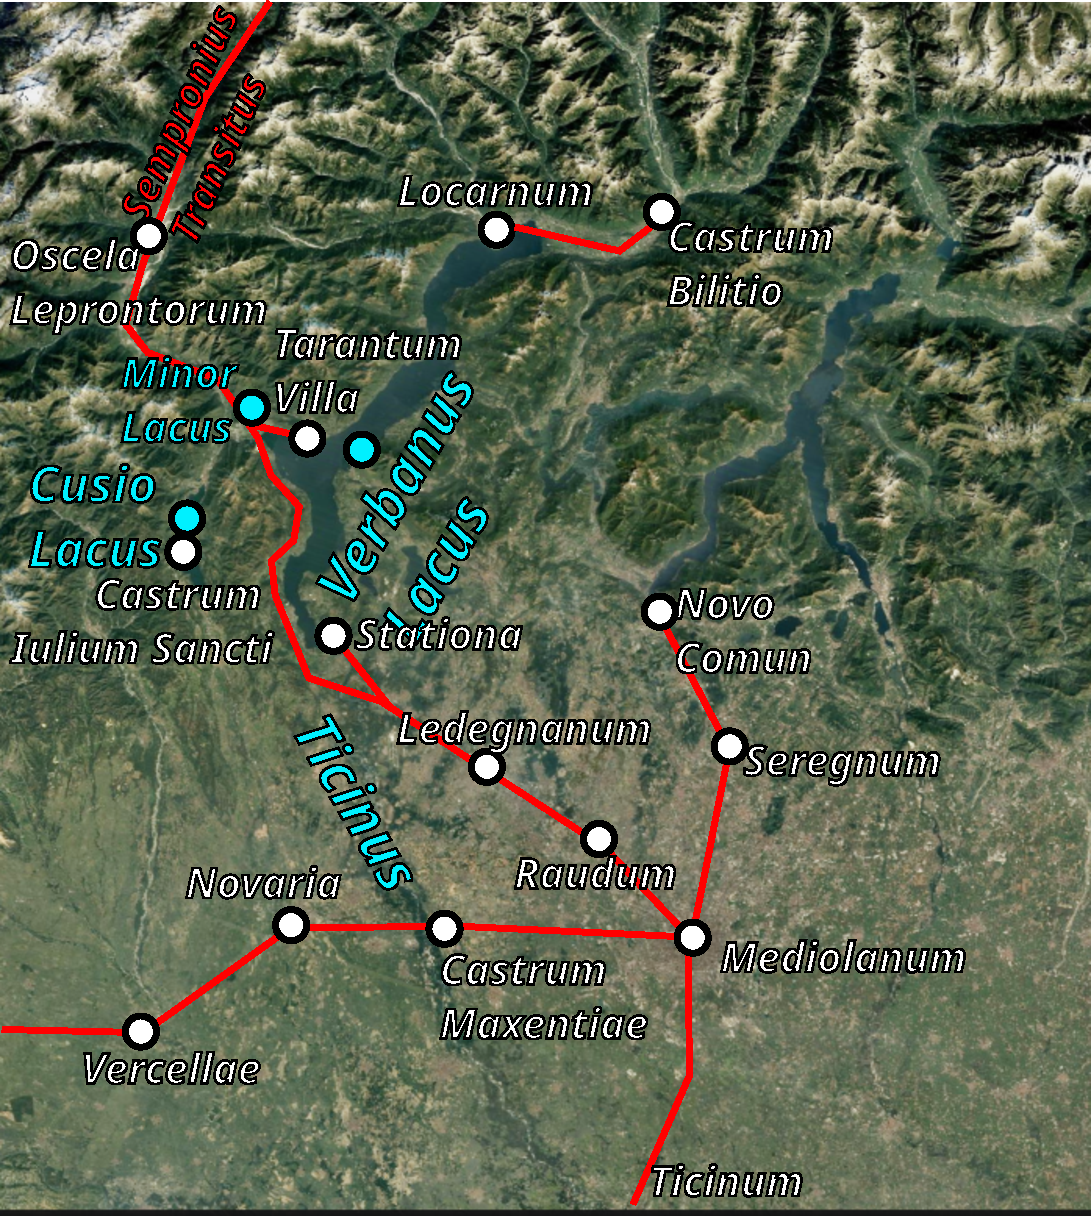
\includegraphics[width=\columnwidth]{img/map-large.pdf}
\end{center}
}

\begin{table}[tb]
\begin{infobox}
\begin{center}
\textsc{Toponimi lacustri}
\end{center}
\smallskip
\begin{tabular}{|m{.45\columnwidth} m{.45\columnwidth}|}
\hline
\textbf{Moderno} & \textbf{Romano}\\
\hline
Lago Maggiore & Verbanus Lacus\\
Lago d'Orta & Cusius Lacus\\
Lago di Como & Larius Lacus\\
Lago di Lugano & Ceresius Lacus\\
Lago d'Iseo & Sebinus Lacus\\
Lago di Varese & Gaviratius Lacus\\
Lago di Mergozzo & Minor Lacus\\ % inventato
\hline 
\end{tabular}
\end{infobox}
\end{table}

\begin{table}[tb]
\begin{infobox}
\begin{center}
\textsc{Lacus Verbanus}
\vspace{1em}
\end{center}
\gradetable{
Conosciuto come Verbanus Lacus dai romani, il nome deriva dalla florida quantit\`{a} di \emph{\objref{Verbena} Officinalis} -- pianta sacra per eccellenza -- che fiorisce sulle sponde del Lacus.
La via per il Lacus \`{e} la Mediolanum - Verbannus, che segue il fiume Olona per poi dipartire verso Ovest fino a Stationa (Toponimo Moderno: Angera).
}{
Camelie e rododendri si aggiungono alla flora delle sponde del Verbano.
Tra i locali, il Lacus Verbanus \`{e} anche noto come Lacus Maximus.
La strada da Stationa a Oscela Lepontiorum non \`{e} lastricata e assomiglia pi\`{u} a un largo sentiero che ad una strada romana vera e propria.
La via poi prosegue fino ai passi alpini.
}{
Nonostante l'impero abbia contribuito in modo significativo alla viabilit\`{a} nella zona, non esiste un ponte per attraversare il Ticinum nei pressi del Lacus.
Il trasporto di persone e beni \`{e} una attivit\`{a} commerciale molto florida nei pressi sulle sponde del Verbanus.
Piccole isole sono presenti in diverse aree del Lacus, nelle quali trovano posto fragili micro-climi sorprendentemente temperati. A monte di questo lacus vi sono diversi specchi d'acqua di minore estensione, tra cui il pi\`{u} noto \`{e} il Cusius Lacus.
}
\end{infobox}
\end{table}

\begin{description}
\item[Augusta Taurinorum] Urbe capoluogo della Transpadana e sede di un distaccamento della Coorte Arcana.
\\Toponimo moderno: Torino.
\item[Castrum Maxentiae] villaggio a ovest di Mediolanum, situato poco distante dalle rive del Ticinum.
Ha una profonda vocazione agricola, anche se \`{e} circondato da paludi.
La sua fortuna la fanno una piccola mansio e il commercio fluviale.
Nonostante il nome possa suggerire una presenza militare sostanziosa, il castrum \`{e} decisamente di modeste dimensioni e prevalentemente presidiato da auxiliares sotto la supervisione di solamente un pretoriano.
\\Toponimo moderno: Magenta.
\item[Castrum Iulium Sancti] Piccola isola sul Cusius Lacus e sede di una comunit\`{a} di rifugiati cristiani.
Da circa due secoli, cristiani di origine greca si sono stabiliti in questa conca e hanno iniziato a soppiantare i riti celtici.
Sebbene la maggioranza degli abitanti sia di fede cristiana, le autorit\`{a} romane hanno imposto ai locali la presenza di un luogo di culto riservato ad una divinit\`{a} romana.
Sebbene sia principalmente di rappresentanza, il compromesso con i cristiani greci venne raggiunto erigendo una piccola edicola votata ad Ecate.
\\Toponimo moderno: Isola di San Giulio.
\item[Cusius Lacus] Piccolo lacus situato a monte rispetto al Verbanus, circa a met\`{a} latitudine in direzione ovest.
Non ha affluenti e il suo uno effluente \`{e} il torrente Strona, immissario del fiume Tocis.
\item[Mediolanum] Urbe a vocazione mercantile situata tra la Transpadana e la Venetia.
Canali guidano le acque del Seveso e del Lambro dentro e fuori Mediolanum consentendo la presenza di un porto fluviale.
Celti della trib\`{u} insubre hanno ancora una modesta influenza in citt\`{a} e nelle aree circostanti.
\\Toponimo moderno: Milano.
\item[Minor Lacus] Specchio d'acqua a ovest del Verbanus Lacus, e poche miglia a sud del Cusius Lacus.
Nonostante disti a circa un miglio di distanza dal Verbanus, in pochi si ricordano della sua esistenza, probabilmente a causa della sua limitata estensione ed importanza.
Sulla sponda nord-occidentale vi \`{e} un piccolo insediamento Lepronto il cui nome sfugge ai pi\`{u}.
\item[Montem Rotundus] Monte che separa il Verbanus Lacus dal Cusius Lacus.\\
Toponimo moderno: Mottarone.
\item[Oscela Lepontiorum] Ultimo posto confortevole prima dei rifugi alpini;
villaggio romano di origine celtica situato al centro della valle Oscela.
Parzialmente nascosti all'impero, si mormora che i sacerdoti dei Leponti pratichino ancora culti druidici in questi luoghi.
\\Toponimo Moderno: Domodossola.
\item[Stationa] Porto lacustre a sud del Lacus Verbanus.
\\Toponimo Moderno: Angera.
\item[Tarentum] Ricca urbe nella Magna Grecia. Famosa per commercio di tessuti.
\\Toponimo Moderno: Taranto.
\item[Tarentum Villa] Villa di campagna sulle sponde del Verbanus lacus.
Ampi terreni coltivati a frutteto la circondano, ma si dice che tra le sue mura si celino opere d'arte molto ricercate.
Residenza estiva di un senatore di Mediolanum avente legami con la urbe di Tarentum, ma tra i locali nessuno conosce esattamente il nome del proprietario.
\item[Ticinum] Urbe costruita sulle sponde del Ticinum a sud-ovest di Mediolanum.
\\Toponimo moderno: Pavia.
\item[Ticinus] Fiume emissario del Verbabus Lacus ed immissario del Padus.
\item[Vehemenia] Borgo abitato da pochi montanari, situato alla foce del Cusius Lacus.
Per molti servizi, dipende da Castrum Iulium Sancti.
\\Toponimo Moderno: Omegna.
\item[Verbanus Lacus] Specchio d'acqua a nord-ovest di Mediolanum. Vedi box a fianco.
\end{description}

%%%%%%%%%%%%%%%%%%%%%%%%%%%%%%%%%%%%%%%%%%%%%%%%%%%%%%%%%%%%%%%%%%%%%%%%%%%%%%%
\lasection{Personaggi}
%

\monster{\tarantasio}{
\emph{Dimensione: 4}
\begin{center}

\includegraphics[width=\columnwidth]{img/tarantasio2.jpeg}
\end{center}
\dvstat{12}
{Danno, Sensibilitas, Ratio}
{De Bello, De Corpore}
{De Corpore (Saltare), Punti Vita}
{36}
\equip{-}{Pelle Squamata (Protezione 6)}
\specialstat{Afferrare, Volo}{Soffio Infuocato, Magnetismo}

\emph{%
Il magnetismo della sua pelle implica che chiunque sia entro i 10 piedi dal drago (3 metri) debba effettuare per ogni tempus un \tiro{Vigor}{6};
nel caso il tiro fallisca, gli oggetti di ferro impugnati dal personaggio finiranno attaccati alla corazza del drago}

Vedi informazioni circa Dracones Cambrici nel manuale Britannia~\cite{britannia_en} a pagina 170.
Questo drago \`{e} particolarmente attratto dalle acque.
Gli piace riposare in acqua e cibarsi di creature marine.
Di recente ha inizato ad attaccare anche ninfe e fauni lungo le rive dei laghi.
\`{E} normalmente una creatura notturna: si sveglia dopo il tramonto e tende a scomparire alle prime luci dell'alba.
}


\npc{\custosmorta}{
Esploratrice della coorte arcana di circa 40 anni.
Ha indagato a Mediolanum e da l\`{i} ha raggiunto la Villa Tarentum di \npcref{\politico}.
Mentre indagava nella spiaggia privata della villa \`{e} stata assalita e mangiata viva da \monsterref{\tarantasio}.
}


\npc{\politico}{
\dvstat{6}
{De Bello, De Corpore, De Magia}
{De Scientia, De Natura, Sensibilitas, Punti Vita}
{Ratio, De Societate}
{12}
Ex-senatore mediolanense in et\`{a} ormai avanzata, ricopre ora la posizione di aedile della citt\`{a}.
Si \`{e} ritirato dal senato per dedicarsi solo alla urbe e alle sue propriet\`{a} terriere.
\`{E} originario, da parte di madre, di una nobile famiglia di Tarantum.
Suo padre era un mercante di Augusta Tarvinorum, e ha ancora molte consocenze in quella citt\`{a}.
A Mediolanum \`{e} benvoluto dai mercanti locali e dalla popolazione.
\`{E} riuscito a convincere la plebe che le sue politiche hanno abbassato i prezzi, anche se i margini di guadagno per i mercanti locali sono corposi.

Sebbene si mormori sia in punto di morte, in realt\`{a} \`{e} semplicemente terrorizzato da quella che crede sia una maledizione che si \`{e} accanita contro di lui.
Si \`{e} barricato nella sua villa di citt\`{a} e non esce nemmeno per lavorare.
Sospetta -- senza giusta ragione -- che degli assassini si preparino a ucciderlo.
}

\npc{\duumvirouno}{
Cliente di \npcref{\politico}.
\`{E} cresciuto a Roma Urbe e conosce abbstanza bene i giochi della politica.
Cerca di stare fuori dalle faccende potenzialmente rischiose come quelle che coinvolgono la cohorte arcana.
Vede la sua posizione come un passo verso la carica di senatore.
%
\`{E} molto grato a \npcref{\politico} per il suo ruolo come aedile della citt\`{a} in quanto si fa carico di gran parte delle decisioni difficili.
}

\npc{\duumvirodue}{
\`{E} cresciuto a Mediolanum ma ha origini transalpine.
Segue le vicende commerciali della citt\`{a} in prima persona.
Prudente e scaltro, vorrebbe diventare senatore prima di \npcref{\duumvirouno} pur essendo pi\`{u} giovane di quasi due lustri.
%
Deve la sua carriera politica alla benevolenza di \npcref{\politico} e spera di godere del suo apoggio per ambire a cariche importanti nella Urbe Aeterna.
}

\npc{\silvano}{
Gran Sacerdote del Grande Tempio di Mediolanum.
Ha divinato a \npcref{\politico} presagi nefasti riguardo l'acqua di Mediolanum.
I presagi nefasti riguardavano anche il commercio cittadino.
Questi presagi potranno essere confermati dai custodes con opportuni rituali.
}

\npc{\druidolepronti}{
\dvstat{8}
{De Bello, De Corpore, De Scientia}
{De Societate, Punti Vita}
{De Natura, De Magia, De Societate (Comandare)}
{16}
Druido a capo della tribt\`{u} dei Lepronti da Oscela Lepontiorum.
Porta al collo un ciondolo di Ambra Nera del Padus.
Convocato dalla trib\`{u} apparsa nel Cusio, ha risposto alla chiamata per discutere con i nuovi arrivati di una potenziale alleanza in chiave anti-romana in memoria della Fratellanza Transnazionale\footnote{Vedi manuale Italia~\cite{italia_it} pagina 161.};
ancora non si \`{e} apertamente schierato.
}

\npc{\prostitute}{
\dvstat{5}
{De Bello, De Scientia, Ratio, Punti Vita}
{De Societate, De Corpore, De Natura}
{Sensibilitas, De Societate (Seduzione)}
{5}
Lucilla Bentigodi e Luciana Bentivoglio.
Cresciute nella povert\`{a}, sono originarie di villaggi poco conosciuti situati sulle rive del fiume Ticinus, ad ovest di Mediolanum.
Hanno lavorato per diversi anni nella zona di Castrum Maxentiae, ma da alcuni mesi il lavoro \`{e} improvvisamente calato e sono state costrette a cercare fortuna presso la grande citt\`{a} di Mediolanum.
Cercano di attrarre clienti nella zona di Porta Romana, ma sembrano non essere abituate alla vita di citt\`{a}.
Non hanno idea di cosa si nasconda dietro il misterioso calo di lavoro, ma sanno che una nuova ``attrazione'' -- chiamata \emph{\npcref{Bocca di Rosa}} dai locali -- le ha mandate fuori mercato.
Disprezzano questa \npcref{Bocca di Rosa} anche se non sanno se esista davvero.
}

\npc{Bocca di Rosa}{
\dvstat{6}
{De Bello}
{Ratio, Punti Vita}
{De Societate}
{12}
Ninfa acquatica particolarmente attiva ed efficace nel destare le attenzioni degli uomini che si accampano nei pressi delle sue acque.
Originaria del Verbanus Lacus, \`{e} stata costretta a migrare a sud a causa di un grosso e vorace predatore alloctono introdotto di recente in quelle acque.
Non \`{e} a suo agio nel clima paludoso del Ticinus.

Se i custodes la cercano, lei tenter\`{a} di sedurre uno o pi\`{u} di loro alla prima notte che trascorreranno nei pressi delle rive del Ticinus.
Chi resister\`{a} al suo fascino, potr\`{a} interrogarla ed ella volentieri avvertir\`{a} il contubernium del pericolo a monte.
}

\npc{\villico}{
Nato e cresciuto sulle sponde di questo lago, ha alle spalle una carriera da pescatore.
Fino a tre lustri fa, era l'organizzatore della gara di pesca locale, poi fu scelto per succedere al defunto villico di Tarentum Villa e da allora si limita a partecipare.
Tra i locali \`{e} anche conosciuto con il nomignolo di \emph{Re d\`{i}i cav\`{e}den}.

Ora gestisce Villa Tarentum per conto di \npcref{\politico}.
\`{E} l'unico tra la servit\`{u} e la popolazione locale a conoscere l'esatto nome del proprietario di questa villa, ma a lui importa poco: per lui \`{e} solo \emph{El Par\'{o}n}.
%
Ha assistito alla scena in cui \npcref{\custosmorta} \`{e} stata uccisa, ma ha dimenticato interamente la scena a causa della \objref{\canzone}.
}

\npc{\ecatina}{
\dvstat{6}
{De Bello, De Corpore, De Societate}
{De Natura, De Scientia, Punti Vita}
{De Magia, Ratio, Sensibilitas}
{12}
Giovane sacerdotessa di Ecate, leggermente scontrosa ma bonacciona.
Decisamente un'anima campagnola con tanta vocazione per la montagna e un po' meno per le persone.
Ecate la ha resa immune all'effetto della \objref{\canzone}.
Per la comunit\`{a} cristiana della zona prova poca simpatia, ma ha un elevato senso del dovere verso il suo ruolo di sacerdotessa.
Quando sono arrivati gli invasori, ha deciso che resistere \`{e} bene ma non morire forse \`{e} meglio.
\`{E} scappata sui monti con un fauno perch\'{e} quest'ultimo non ha troppe esigenze ma soprattutto fornisce grandi soddisfazioni a letto.
Si ricorda dell'arrivo degli invasori e di come hanno conquistato il villaggio e decimato la popolazione cristiana tramite sacrifici umani alle loro divinit\`{a} impure.

La sua relazione con un fauno la ha portata ad abbandonare alcuni dei suoi doveri sacerdotali, tra cui la gestione del luogo sacro, ora in mano agli invasori.
}
%\eject

%%%%%%%%%%%%%%%%%%%%%%%%%%%%%%%%%%%%%%%%%%%%%%%%%%%%%%%%%%%%%%%%%%%%%%%%%%%%%%%
\lapart{Fatti antecedenti}
Durante il periodo della conquista romana della Britannia, una trib\`{u} celtica decise di combattere Roma seguendo la tattica di Annibale.
Mentre i romani avanzavano sull'isola, la trib\`{u} ha deciso di passare alle loro spalle attraversando un luogo sottile.
Il loro piano originario era quello di radunare altre trib\`{u} della \emph{Fratellanza Transnazionale}\footnote{Vedi manuale Italia~\cite{italia_it} a pagina 162.} per cogliere di sorpresa le truppe romane dove meno se lo aspettano: in Italia.
Tuttavia, questo piano \`{e} stato rovinato da qualche scherzetto dei fatui, i quali hanno trattenuto la trib\`{u} nel reame fatato pi\`{u} a lungo del previsto.

La trib\`{u} ha viaggiato dalla Britannia Secunda alla Gallia Cisalpina attraverso il reame fatato nell'arco di tempo di pochi giorni di cammino -- o questo a loro \`{e} sembrato!
Nella realt\`{a}, sono trascorsi circa quattro secoli.
Al loro seguito portano un draco ammaestrato che il loro druido ha intenzione di usare come arma contro Roma proprio come Annibale port\`{o} con s\`{e} gli elefanti.

Questa trib\`{u} \`{e} riapparsa da un luogo sottile nei pressi del Cusius Lacus circa due mesi fa.
L\`{i} hanno incontrato la comunit\`{a} locale di cristiani e un presidio di quattro legionari assegnati al monitoraggio della situazione sul Cusio.
Il legionario di guardia \`{e} morto sul campo.
Un secondo legionario \`{e} stato intercettato dal drago sulle sponde del Verbanus, nei pressi di Tarantum Villa, prima che potesse riportare a Roma il messaggio di allarme.
Alcuni servitori della villa hanno assistito alla scena e hanno pensato si trattasse del drago Mediolanensis \emph{Tarantasium}.
Il terzo legionario ha seguito la sorte del secondo, a distanza di tre settimane.
Il quarto sta pregando gli d\`{e}i che i rinforzi da Roma arrivino presto.

Sebbene nessun legionario sia riuscito a fare rapporto, il \emph{vilicus} ha inviato un messo a Mediolanum per allertare il proprietario della villa.
Data la situazione caotica e un passaparola poco accurato, il senatore Quinto Lavinius Lycaeus -- proprietario della villa -- non ha capito molto bene la situazione.
Il senatore ha allertato la cohorte arcana di Augusta Taurinorum e ha raccomandato molta discrezione.
\custosmorta ha iniziato ad indagare nella zona su indicazione del senatore, ma \`{e} anch'ella finita divorata da Tarantasium.

La comunit\`{a} cristiana \`{e} stata decimata, e gli unici sopravvissuti abitano in baite isolate sui fianchi delle montagne.
Tra loro, una sacerdotessa di Ecate ha abbandonato il suo tempietto sulle rive del lago e ha iniziato una nuova vita in una baita sul Minor Lacus, accompagnata da un fauno.

Il drago Tarantasium stesso ha subito qualche sortilegio durante la sua permanenza nel reame fatato, forse una maledizione di un fatuo oscuro che gli ha annebbiato la mente, ed ora non risponde pi\`{u} ai comandi del druido, il quale fatica a contenere la sua furia.
Il drago attacca regolarmente la fauna locale, esseri umani e creature mistiche incluse.

Ninfe e fauni che popolano le sponde del Verbanus sono ora sotto assedio -- o hanno gi\`{a} migrato -- per sfuggire alla furia divoratrice di Tarantasium.
I pesci del Verbanus e del Cusius sono stati divorati o sono migrati a valle.
Alcuni pescatori sono scomparsi, ma in pochi sembrano essersene accorti.
Il Ticinus ha ricevuto una migrazione anormale di creature acquatiche e il suo ecosistema \`{e} stato alterato.
Morie di pesci e altri problemi da sovraffollamento delle sue acque si manifestano lungo tutto il suo corso fino al Padus.

%%%%%%%%%%%%%%%%%%%%%%%%%%%%%%%%%%%%%%%%%%%%%%%%%%%%%%%%%%%%%%%%%%%%%%%%%%%%%%%
\part{Passacarte}

\section{Da Roma verso Nord}
%
Il viaggio da Roma verso il Padus \`{e} generalmente privo di pericoli.
Le strade sono frequentate da mercanti, viandandi e pellegrini di ogni tipo.
Manipoli di legionari pattugliano ciascuno una mansio a intervalli regolari.
Attraversando il Padus e/o il Ticinus, uno dei custos ricever\`{a} il sogno premonitore \dreamref{Un Pericolo dal Passato}.

\dream{Un Pericolo dal Passato}{
Grani di sabbia scendono da una clessidra, in modo lento ma costante.
Ad un tratto un lampo mostra l'immagine di Enea.
Lentamente l'immagine si fa piccola, sempre pi\`{u} piccola, come un granello di sabbia.
L'immagine di Enea a quel punto attraversa la clessidra, si adagia sul fondo assieme ad altri granelli di sabbia, e l\`{i} vi resta.
%
Poco dopo la scena si ripete. Un altro lampo mostra l'immagine di Romolo, il quale anch'egli rimpicciolisce assieme agli altri granelli di sabbia.
L'immagine di Romolo si adagia anch'essa sui granelli di sabbia e l\`{i} vi resta.
La scena si ripete ancora con l'immagine di Cesare. Stessa sequenza.

Passano altre immagini, di grandi eroi al servizio di Roma, cos\`{i} come anche le immagini di grandi condottieri che Roma ha temuto.
Passano le immagini di Annibale, Vercingetorige, e altri volti dai lineamenti barbari ma il cui nome sfugge alla memoria.
Ad ogni volto romano, una sensazione di orgoglio e rasserenamento coglie il sognatore.
Ad ogni volto ostile a roma, una sensazione di pericolo e inquietudine coglie il sognatore, che si rasserena poi al passaggio di questa immagine attraverso la clessidra.

Ad un tratto, un volto sconosciuto genera una sensazione di inquietudine che non si calma.
Il granello di sabbia non passa attraverso la clessidra ma scompare nel nulla.
Altri granelli di sabbia passano attraverso la clessidra, ma la sensazione di inquietudine permane.

Ad un tratto il custos si sveglia sempre con il senso di inquietudine in cui dormiva.
Alla prima occasione in cui lo stesso custos sognatore osserver\`{a} una coppa o una bacinella di acqua di fonte, noter\`{a} un granello di sabbia lentamente cadervi al centro.
}

Interpretando questo sogno si potr\`{a} dedurre che:
\gradetext{
La clessidra rappresenta lo scorrere del tempo, e il volto inquietante \`{e} un nemico che Roma non ha ancora sconfitto.
}{
La sparizione del granello indica che il pericolo ha abbandonato questo mondo, ma non che rappresenti una minore minaccia solo per questo.
}{
La riapparizione del granello la mattina seguente indica che il pericolo \`{e} ritornato, ed \`{e} riapparso in mezzo o in prossimit\`{a} di acqua dolce.
}

Nei fascicoli che i custos trasportano, potranno trovare informazioni circa l'essitenza del reame fatato e dei luoghi sottili.\footnote{Vedi pagina 127 nel manuale Britannia~\cite{britannia_en}.}

Durante il tragitto, i custodes potranno osservare episodi di lieve squilibrio naturale nei pressi del Ticinus.
Tuttavia, solo una attenta analisi potr\`{a} rivelare il sovraffollamento ittico delle acque.
Se i custodes decidono di passare senza fermarsi, noteranno sono dei generici presagi nefasti che possono essere facilmenti fraintesi per avvenimenti naturali.

\section{Augusta Tarvinorum}
%
Alla sede della cohorte arcana di Augusta Tarvinorum si rallegrano dell'arrivo dei fascicoli di aggiornamento, anche se richieder\`{a} loro diversi giorni di studio per analizzarli.
Senza indugio, il magister esprime la sua preoccupazione per la custos mancante e vi incarica di andare a Mediolanum a indagare.

Il magister mostra ai custodes una lettera arrivata da un politico mediolanensis circa un mese fa.
\emph{
\say{Caro magister, vi scrivo con rispetto per richiedere assistenza.
Presagi nefasti mi perseguitano da giorni, i sacerdoti sono inquieti, e ora sembra che anche la mia servit\`{u} pi\`{u} fidata sia vittima di pazzia.
I sacrifici agli d\`{e}i non sembra siano bastati.
Ho mobilitato le guardie cittadine ma nulla di inusuale \`{e} stato trovato.
Perch\'{e} gli d\`{e}i sono adirati?
Se questa maledizione non vi ha ancora raggiunto, vi imploro di aiutarmi a fermarla.}
}

Un rituale eseguito ad Augusta Tarvinorum ha verificato che gli d\`{e}i sono veramente preoccupati, ma non adirati con Mediolanum o con i suoi cittadini.
Il magister ha quindi inviato \npcref{\custosmorta} -- esperta custos del cursus exploratorius -- per indagare cosa sta davvero succedendo a Mediolanum tuttavia non ha ricevuto pi\`{u} notizie da quando \`{e} partita.

Il magister fornisce ai custodes il nome del politico -- \npcref{\politico} -- e raccomanda discrezione.

\section{Arrivo a Mediolanum}
%
\monster{\balordi}{
Sono contadini, tutti molto giovani.
Si lamentano che le importazioni di grano dall'Egitto hanno ridotto in povert\`{a} i contadini locali.
In realt\`{a}, questi sono gli eredi di un latifondista deceduto di recente -- Ancus Salvidius Regillus -- e i loro amici e compagni di bevute.
Questi non hanno mai imparato in quale mese seminare i cereali prima che Ancus Salvidius Regillus prematuramente scomparve.
Ne consegue che sono almeno un paio d'anni che ottengono raccolti molto scarsi.

Per le caratteristiche dei suoi membri, si consiglia di utilizzare le statistiche -- leggermente modificate -- di \emph{Contadini e Pastori}\footnote{Vedi pagina 147 del Manuale Base~\cite{corebook_en}.}.

\dvstat{5}{De Bello, Ratio, De Natura (Agricoltura)}{De Corpore, Punti Vita, Sensibilitas}{De Natura (Allevamento)}{10}
\equip{Arma improvvisata (Danno: 4)}{Nessuna}
}

\object{Idrografia Mediolanensis}{
\begin{center}
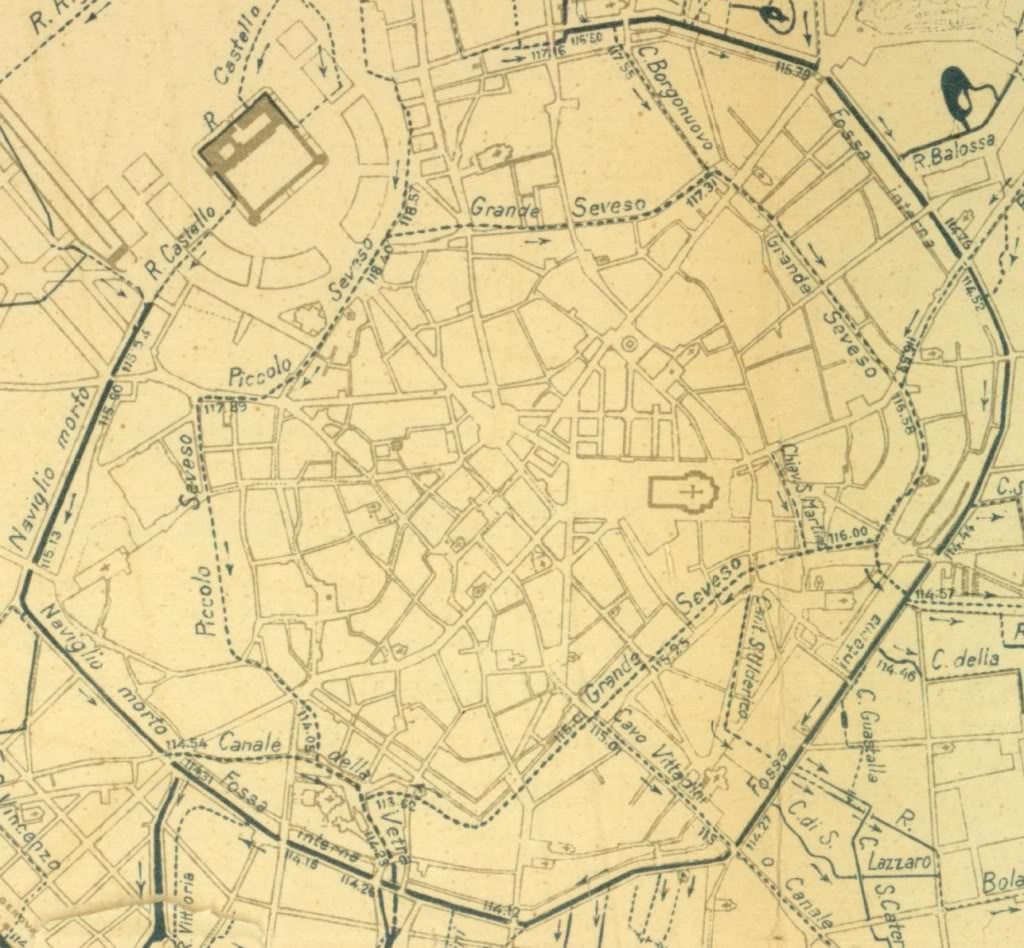
\includegraphics[width=\columnwidth]{img/Milano.jpg}
\end{center}

Una fitta rete di canali navigabili permette il trasporto di merci via acqua in vari punti del centro, vi \`{e} perfino un porto fluviale!

Un piccolo torrente -- Nirone -- passa attraverso il centro e fu il primo corso d'acqua ad essere deviato per accomodare le necessit\`{a} di Mediolanum.
La maggior parte dell'acqua, tuttavia, viene da due canali (Grande Seveso e Piccolo Seveso) che attingono acqua dal fiume Seveso (a est) tramite il Naviglio Martesana.
In aggiunta, il fiume Olona ad ovest ed il torrente Lambro meridionale sono stati deviati per portare acqua in centro e facilitare il trasporto fluviale.

Il torrente Nirone e il Naviglio Vettabbia portano l'acqua fuori da Mediolanum rispettivamente al Olona (a sud-ovest) e al Lambro (a sud-est).

\smallskip
\footnotesize
\emph{Nota: rispetto all'immagine qui sopra, il Naviglio Grande non esisteva ancora in epoca romana, mentre il Naviglio Pavese esisteva solo nell'ultimo tratto.}
}

In citt\`{a} sembra tutto scorrere regolarmente, ad eccezione di tre situazioni:
\begin{enumerate}
\item \npcref{\politico} \`{e} sparito dalla vita pubblica.
Si dice sia malato.
\item nella zona meridionale della citt\`{a}, delle prostitute campagnole sembrano fare fatica ad adattarsi alla vita cittadina.
\item la \monsterref{\balordi} protesta in piazza, forte di circa 20-25 membri.
\end{enumerate}

Dicerie in citt\`{a}:
\begin{itemize}
\item La citt\`{a} ha una ricca offerta artistica, un teatro, un anfiteatro, e un circo a poca distanza l'uno dall'altro.
\item Diversi operai hanno di recente lavorato per conto del comune in opera di manutenzione di canali, terme, acquedotti, e perfino latrine.
Si dice che le latrine siano ora pi\`{u} pulite della camicia di un legionario.
\item Le nuove \npcref{\prostitute} sono molto attraenti -- e anche brave! -- ma non sanno nemmeno contare i soldi.
A volte paghi il doppio, a volte paghi la met\`{a} della tariffa, ma per quanto sono brave non importa...
\item La citt\`{a} ha una minoranza di cristiani leggermente pi\`{u} numerosa di altre citt\`{a} imperiali.
Qui si trova un vescovo che coordina e supervisiona numerose comunit\`{a} sparse per le campagne.
I romani preferiscono ebrei e cristiani agli ancora numerosi culti celto-druidici diffusi in questa provincia dell'impero.
\item I ricchi della zona hanno tutti una residenza estiva sul Verbanus o sul Larius.
Quelli un po' meno ricchi, la hanno sul Sebinus.
\end{itemize}


Le \npcref{\prostitute} si mostrano diffidenti, ma molto imbranate.
Sar\`{a} sufficiente un \tiro{De Societate (Bassifondi)}{3} per estorcere loro le seguenti informazioni:
\gradetext{
Sono arrivate a Mediolanum da un paio di settimane perch\'{e} nelle loro campagne non si lavora pi\`{u} come una volta.
}{
Sono originarie di Castrum Maxentiae.
Da un paio di mesi, in quel paese e nelle campagne attorno si vedono sempre pi\`{u} viandanti ma quasi nessuno si ferma pi\`{u} a passare la notte con loro.
}{
Secondo loro, \`{e} tutta colpa di \npcref{Bocca di Rosa}, un demone che infesta il paese e ruba le energie degli uomini.
-- \say{L'impero dovrebbe proteggerci da questi demoni... e invece noi paghiamo le tasse senza nemmeno poter lavorare! Se foste disposti ad aiutarci, per voi lavoreremmo anche gratis.}
}

Il gran sacerdote \npcref{\silvano} si mostra disponibile nei confronti dei custodes.
Potr\`{a} riferire di aver divinato dei cattivi presagi ed un pericolo imminente -- o forse gi\`{a} in essere -- relativamente all'acqua di Mediolanum.
\npcref{\silvano} non ha predetto alcuna maledizione nei confronti di \npcref{\politico} ma quest'ultimo sembra essersene convinto da solo.
Se i custodes insistono, \npcref{\silvano} dice -- \say{So che \`{e} successo qualcosa nella sua residenza estiva ma non conosco i dettagli.}

% proteste in piazza - contadini protestano
% commercianti sono contenti
% alcuni commercianti hanno lieve preoccupazione per carenza di Emmentalinensis
% nemici: associazione la spiga, figli di contadini diventati poveri a causa delle importazioni di grano dall'egitto

\section{L'imboscata}
%
Nel caso in cui i custodes si facessero riconoscere in pubblico come pretoriani o rappresentanti dell'Impero, questi subiranno una imboscata da parte della \monsterref{\balordi}.
Questa imboscata avviene la prima notte in cui i custodes non dormono in un luogo fortemente sorvegliato.
L'obiettivo degli attaccanti \`{e} di sequestrare qualcuno di importante per poi negoziare dazi sul grano egiziano.

I membri della \monsterref{\balordi} attaccano a mani nude con l'obiettivo di immobilizzare i costodes e sono in numero pari al doppio dei custodes (\textbf{2:1}).

%%%%%%%%%%%%%%%%%%%%%%%%%%%%%%%%%%%%%%%%%%%%%%%%%%%%%%%%%%%%%%%%%%%%%%%%%%%%%%%
\part{Acque Irritate}
%
\section{Indagini a Mediolanum}
%
Con opportune indagini, i custodes scopriranno che:
\begin{itemize}
\item la \monsterref{\balordi} \`{e} nata da poco e -- stando all'opinione popolare -- sono dei perditempo che cercano di fare rumore solo per far eleggere a duumviro uno della loro famiglia di contadini.
Fanno paura solo perch\'{e} fanno rumore.
%
\item \npcref{\politico} ha ordinato diverse ispezioni dei acquedotti, canali, fogne, e bagni termali della citt\`{a} -- opera non da poco, considerata la fitta rete idrica di Mediolanum -- ma nulla di anormale \`{e} stato trovato.
%
\item \npcref{\politico} ha stanziato delle pattuglie sulle acque del Larius Larius e del Gaviratius Lacus.
%
\item \npcref{\duumvirouno} e \npcref{\duumvirodue} sono preoccupati per lo stato di salute -- fisica e mentale -- di \npcref{\politico}.
%
\item \npcref{\duumvirodue} sta indagando su inaspettato calo di approvvigionamento di Emmentalinensis -- ed altri formaggi elvetici -- verificatosi negli ultimi due mesi, sembra che non arrivino pi\`{u} tanti mercanti da Oscela Leprontorum.
%
\item \npcref{\politico} ha diverse propriet\`{a}: una villa sul mare a Tarantum chiamata \emph{Verbanus Villa}, e una villa sul Lacus Verbanus chiamata \emph{Tarantum Villa}.
%
\item qualcosa di sovrannaturale sta davvero succedendo a Castrum Maxentiae e dintorni, ma -- per il momento -- non si tratta di nulla di preoccupante.
Diversi uomini hanno preso abitudine a campeggiare spesso lungo i fontanili e i corsi d'acqua in zona.
%
\item le acque del Ticinus sono diventate molto pi\`{u} pescose, soprattutto nel tratto settentrionale, anche se alcuni pescatori sono preoccupati per la qualit\`{a} del pesce dato che si sono verificate diverse mor\`{i}e di pesci in quelle zone.
\end{itemize}

\section{Mediolanum - Verbanus}
%
\dream{\ninnananna}{
%
Una sensazione di nostalgia ti avvolge, la testa sembra muoversi seguendo una forza pi\`{u} grande che accompagna tutte le oscillazioni con gentili movimenti ad arco.
Vieni cullato/a dolcemente come un genitore culla un figlio.
Ti concentri per capire cosa accade attorno a te, ma non hai le forze o la voglia per fare altro che cullare gentilmente al dondolio a cui sei soggetto.
L'udito parzialmente ti ritorna e inizi a percepire della musica.
Non sai dire da dove viene, ma ti rasserena.
Non sai dire chi la suona, ma ti conforta.
Non sai riconoscere la melodia, ma ti pare una ninna nanna.
Lunghe note poco distanziate, un tempo molto lento, e la convinzione che a suonare c'\`{e} sicuramente qualcuno della tua Gens che vuole solo il tuo bene.

Riesci a catturare qualche frammento di immagine.
Ti trovi da solo/a, in una stanza vuota, accanto ad un focolare che ti scalda.
Sei in una tinozza di legno, a mollo, rilassando le tue membra in acqua tiepida mentre stai lavando il sudore dalla tua pelle.
La musica viene da appena fuori la stanza, hai la sensazione che ci sia qualcuno, una persona, a suonare.
In quel momento, capisci che quella persona non \`{e} qualcuno che conosci e inizia a sentire una sensazione di inquietudine.
%
L'inquietudine si trasforma presto in un senso di irritazione, disagio, e pericolo imminente.
Un rumore di passi si avvicina, una figura incappucciata dalla penombra sbircia dalla porta verso di te.
Ti vede.
Sorride, ma con un ghigno di disprezzo la sua attenzione volge oltre la tua umana presenza.
Oltre la soglia, l'incappucciato si allontana.

Sei turbato, ma allo stesso tempo sollevato perch\'{e} la direzione presa da questa figura non \`{e} apertamente ostile, non in questo momento almeno.
La sensazione di sollievo dura poco.
Dalla stessa soglia, all'improvviso un tonfo.
La tinozza trema.
Rialzi lo sguardo e noti tre artigli, conficcati nel muro, ciascuno mezzo metro dentro la stanza, ma chiss\`{a} quanto pi\`{u} lunghi prima della carne che li porta.
Il cuore ti tradisce e salta un battito.
Un rumore di striscio e trascinamento segue.
Fuori dalla stanza, nella luce proiettata dalle candele nella stanza scorgi quella che ti sembra una coda di serpente che striscia allontanandosi.
Hai paura e ti svegli.
}

Tutto procede regolarmente fino a Stationa.
Lungo la via, circa a met\`{a} strada, i custodes sognano la \dreamref{\ninnananna}.
I custodes incontrano abitanti e mercanti -- tutti molto riservati -- ma nessun mercante che provenga da oltre Stationa.
Interpretare il sogno porta al seguente responso:
\gradetext{%
Un pericolo \`{e} apparso e si nasconde in attesa di colpire.
Il pericolo \`{e} rappresentato da uno o pi\`{u} uomini, con al seguito creature a voi sconosciute.
}{%
Diffidate della musica che tranquillizza e sembra familiare perch\'{e} in realt\`{a} cela un pericolo.
La tinozza rappresenta un bacino d'acqua, forse una lago.
Il focolare indica un insediamento civilizzato, forse romano forse no, sicuramente rurale.
}{%
La parete invece simbolizza un ostacolo -- forte artificiale o forse naturale -- che separa, maschera ed ostruisce la visuale impedendo di vedere il pericolo se non a tratti.
La porta rappresenta uno spiraglio, un passo, un vallo, che offre una limitata visuale sul pericolo.
}

Al castrum di Stationa i custodes vengono informati di una relativa calma innaturale sul lago, e sulle sue sponde.
I custodes che superano un \tiro{Sensibilitas}{9} avranno l'impressione che le guardie da queste parti sono abbastanza menefreghiste e non abbiano molti contatti con la popolazione locale a nord del loro castrum.

\section{Verbanus}
%
\object{Verbena}{
I Romani -- ma anche popoli precedenti -- identificano la verbena comune o \emph{Verbena Officinalis} come pianta sacra per eccellenza, un'erba ``miracolosa'', una panacea universale.
Usata nei rituali per le sue propriet\`{a} psicoattive e le cui fibre venivano intrecciate fino a formare una corona da vestire.
Caratteristiche comuni anche per l'alloro, altra pianta sacra dell'antica Roma.

Chimicamente parlando, la verbena possiede propriet\`{a} antidepressive, antinevralgiche, spasmolitiche, febbrifughe, antinfiammatorie; inoltre ha propriet\`{a} emollienti e rinfrescanti.
}

Da Stationa non si attraversa il lago, la corrente \`{e} troppo forte e c'\`{e} elevato rischio di impantanarsi con la zattera.
Bisogna scendere a valle poche miglia per trovare un molo a cui sono ancorati alcuni battelli per compiere la traversatra sul Ticinus.
Da l\`{i}, la Mediolanum - Verbanus riparte costeggiando il lago sulla sponda ovest in direzione del Transitus Sempronius.
Una volta attraversato il Ticinus, i custos potranno udire al tramonto il suono della \objref{\canzone}, la stessa melodia del sogno \dreamref{\ninnananna} provenire da oltre i monti ad ovest.

Il Verbanus presenta un piccolo arcipelago di tre isole, ciascuna delle quali ha un piccolo molo.
La pi\`{u} grande ha anche una struttura in legno: probabilmente rimessa per le barche.
Dalla riva non si capisce bene se ci sia altro su queste isole, o solo vegetazione boschiva.

\object{\canzone}{
%
Questa particolare melodia, quando viene suonata dalle cornamuse druidiche britanne, ha il potere di calmare gli animi di chi ascolta e annebbiare le loro menti.
Se chi ascolta fallisce un \tiro{Ratio}{6}, la canzone fa scordare gli avvenimenti pi\`{u} traumatici del giorno passato.
}

La sponda orientale del lacus \`{e} prevalentemente acquitrinosa e di difficile percorrenza, in special modo nella parte meridionale del lago.
Gli insediamenti principali si trovano sulla sponda occidentale, cos\`{i} come anche la maggior parte delle ville.

Nonostante la presenza di modeste ville appartenenti ad illustri personaggi locali, il territorio risulta decisamente brullo e scarsamente popolato.
\`{E} evidente che anche tra i nobili e ricchi non sono in molti a desiderare una villa in questi luoghi, o forse anche solo a conoscere questi luoghi.

\object{Gli insediamenti del Verbano}{
\begin{center}
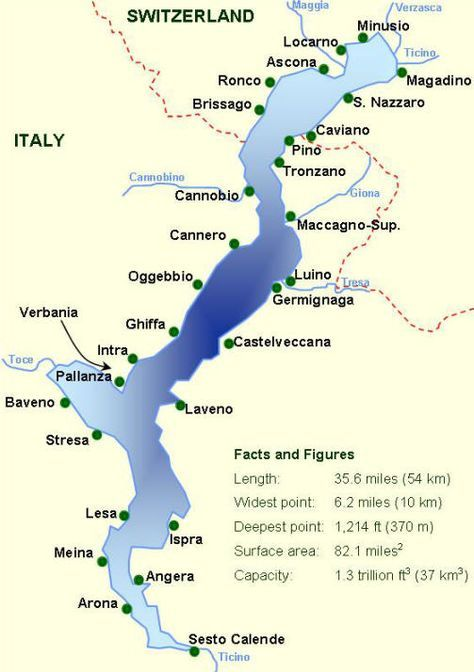
\includegraphics[width=\columnwidth]{img/Verbano.jpg}
\end{center}
\emph{\footnotesize Nota: Questa immagine denota toponimi moderni.}
}

\monster{\aquitani}{
\dvstat{6}
{Ratio, De Magia, De Scientia}
{De Corpore, De Natura, Sensibilitas, Punti Vita}
{De Bello, De Corpore (Marciare)}
{12}
\equip{Spada Celtica (Danno 8), Arcus (Danno 6)}
{Scudo piccolo (Parata +1)}
}

\monster{\druidoaquitano}
{\dvstat{6}
{De Bello, De Corpore}
{De Scientia, Punti Vita, Ratio}
{De Magia, De Natura, Sensibilitas}
{12}
\equip{Falcetto (Danno 4)}
{--}
}

Sulle sponde del Verbanus, i custodes incontreranno un gruppo di \textbf{1:1} \monsterref{\aquitani} impegnati a scortare un \monsterref{\druidoaquitano} verso Castrum Iulius Sancti.
Se riescono ad accorgersi della loro presenza senza essere visti, potranno decidere se tendere una imboscata, affrontarli apertamente, o eluderli senza farsi vedere.
Questi sono diretti verso Castrum Iulium Sancti.
Sebbene il sentiero pi\`{u} veloce dall'Aquitania al villaggio non passi lungo il lago bens\`{i} dietro i monti, quella via \`{e} nota solo ai locali, mentre la via lungo il Verbanus \`{e} nota a molti, incluse tutte le trib\`{u} celte.

\section{Tarentum Villa}
%
La villa \`{e} decisamente lussuosa per i canoni locali e degna di un aristocratico di Mediolanum ma risulta tuttavia spartana nei decori se comparata con le ville di Roma o altre grandi citt\`{a}.
Questa sorge su una piccola collina rocciosa affacciata sul lago.
Nei giorni non troppo nebbiosi, dalla villa si possono vedere due delle tre isole sul Verbanus, perlopi\`{u} disabitate.
L'altura sui cui questa villa si trova, assicura resistenza alle onde e alle piene pur consentendo accesso alla riva.
Dalla collina infatti, tramite una piccola rampa, si arriva ad una spiaggia di ciottoli equipaggiata con un piccolo molo.
Al molo sono ormeggiate due barche a remi, mentre una terza \`{e} in secca, parzialmente coperta da una struttura in legno e avvolta in teli e coperte.
Un muro di cinta avvolge la spiaggia fino a chiudersi all'interno incontrando le acque del lago alla fine della spiaggia privata.

La struttura tipica della villa romana in questo caso \`{e} modificata per consentire l'accesso alla rampa che porta alla spiaggia tramite il cortile interno.
I terreni immediatamente adiacenti alle mura sono coltivati a frutteto, ma i filari sono pochi, pi\`{u} in l\`{a} castagni secolari dominano il territorio.

All'interno della villa, due persone la mantengono: il villico \npcref{\villico} e un servitore.
Un secondo servitore dovrebbe trovarsi nella villa ma non sanno dove sia.
Sia il villico che il servitore non si ricordano di cosa successe mesi fa e non hanno memoria del passaggio di trib\`{u} di celti in zona.

La spiaggia privata della villa \`{e} dove \monsterref{\tarantasio} ha catturato e mangiato \npcref{\custosmorta} poco dopo che questa arriv\`{o} sul luogo.
Con un \tiro{De Natura (Cacciare)}{9} i custodes troveranno tracce di lotta sulla spiaggia come tracce di bruciature causate dall'alito di fuoco di \monsterref{\tarantasio} o graffi causati dai suoi artigli.

All'interno della villa, un \tiro{De Scientia (Indagare)}{6} riveler\`{a} che:
\gradetext{
La stanza del servitore mancante \`{e} poco in ordine.
Sembra che qualcuno abbia arraffato di corsa alcuni oggetti e poi abbia lasciato la stanza.
Da questa stanza, una piccola feritoia nel muro si affaccia sulla spiaggia.
}{
Qualcuno ha iniziato a spostare i documenti nello studio di \npcref{\politico} ma -- non trovando nulla di interessante -- ha desistito senza rimettere a posto.
}{
Nella stanza del servitore mancante ci sono tracce di erbe sacre bruciacchiate e uno specchio che vi sembra familiare.
Forse qui qualcuno ha eseguito un rituale di speculum.
}

\dream{\confratelli}{
Sogni di essere ad una tavolata in famiglia.
Sei seduto accanto a tua moglie al centro della tavolata.
Accanto a voi ci sono dodici vostri figli che siedono sei alla vostra destra e sei a sinistra.
State pranzando, i servitori portano cibo per tutti alla tavola.
I vostri figli aspettano tutti un vostro cenno prima di iniziare a mangiare ogni portata.

Ad un tratto, entra nella sala una figura incappucciata che cattura l'attenzione di alcuni.
Noti che quattro dei tuoi figli si sono alzati per andargli incontro.
Lo salutano, lo abbracciano, lo baciano come si fa con un fratello che non si vede da tempo.
In quel momento, l'incappucciato estrae da una tasca un sacchetto di sabbia e lo svuota sul pavimento.
Con l'ausilio di un bastone, disegnano sulla sabbia un simbolo.
\begin{center}

\includegraphics[width=.5\columnwidth]{img/celtic-knot.pdf}
\end{center}
I cinque si abbracciano e si siedono ad un tavolo separato.
L'ultimo arrivato abbassa quindi il cappuccio rivelando una rossa chioma, si volta verso di te e lancia un coltello in faccia.
Con la lama a un soffio dal naso, ti svegli.
}

Alla prima notte dopo la visita alla villa, un custos riceve il sogno \dreamref{\confratelli}.
Interpretare il sogno porta al seguente responso:
\gradetext{
La ricomparsa di un nemico di Roma sta sollevando una rivolta contro Roma.
Il sognatore si ricorda il simbolo disegnato e capisce che \`{e} di origine celtica.
}{
La tavolata rappresenta l'impero con i suoi leali sudditi.
Il numero dodici simboleggia la completezza e non rappresenta un numero esatto.
Il disegno \`{e} simbolo di una antica alleanza tra i popoli celtici.
}{
Il tavolo a cui si siedono rappresenta la fondazione di una nazione nemica di Roma e formata da sole popolazioni di trib\`{u} celte.
La rossa chioma \`{e} tipica di trib\`{u} celte di origine britanna.
}


\section{Lungo il Tocis}
%
\monster{\predatore}{
\dvstat{4}
{Danni, Punti Vita}
{De Corpore}
{De Bello, Sensibilitas}
{4}
\specialstat{Picchiata\footnote{All'inizio del combattimento oppure nel caso in cui nel tempus precedente il PNG non era ingaggiato, se il PNG risulta attaccante, in quel tempus il suo moltiplicatore del Danno \`{e} aumentato di 1.
Dopo la picchiata, la creatura prosegue il combattimento normalmente},
Sensi acuti\footnote{La difficolt\`{a} dei tiri per tendere imboscate a oppure
per nascondersi da questo PNG, \`{e} aumentata di 1 livello.},
Volo\footnote{Durante il combattimento pu\`{o} sempre scegliere quale avversario ingaggiare e come azione nel proprio tempus pu\`{o} liberamente passare da ingaggiata a non ingaggiata (e viceversa) senza alcun tiro.
A meno che non stia affrontando altre creature volanti, pu\`{o} rimanere nella posizione non ingaggiata quanto desidera, o fuggire dal combattimento senza effettuare tiri.
Grazie a questa abilit\`{a}, la creatura pu\`{o} quindi effettuare una Picchiata ogni 2 tempus, sfruttando il tempus intermedio per tornare nella posizione non ingaggiata.}
}{--}
Questi predatori sono disturbati dall'alterazione dell'ecosistema locale.
La presenza di \monsterref{\tarantasio} ha ridotto la presenza di prede e aumentato i pericoli per il loro nido.
}

La via segue il corso del torrente Tocis ed \`{e} un alternarsi di sentieri di montagna e pantani paludosi.
Il tragitto \`{e} solo poche miglia ma l'attraversamento impiega diverse ore, a causa della morfologia e delle condizioni del terreno.
Lungo la strada, una inusuale vista di interi alberi sradicati accompagna i custodes dal Verbanus al Cusius lungo le rive del Tocis.

All'ingresso della valle del Tocis, \monsterref{\druidonemico} ha posizionato un Sigillum Patronum\footnote{Vedi manuale Britannia~\cite{britannia_en} a pagina 155.} che avvisa il druido dell'arrivo di un gruppo ostile numeroso quanti sono i custodes.
Questo sigillo \`{e} nascosto e i custodes potranno notare qualcosa solo se superano un \tiro{Sensibilitas}{6}:
\gradetext{%
Diverse rune sono incise sulle rocce lungo il passaggio.
Alcune sembrano antiche, altre pi\`{u} recenti.
\`{E} difficile distinguere cosa ci sia scritto anche a causa di evidenti segni di depistaggio, \`{e} come se qualcuno o qualcosa abbia abraso intere porzioni di queste rune.
}{%
Sembrano messaggi di monito scritti in un alfabeto celtico, ma non \`{e} lo stesso dei Lepronti.
Alcune parti di questo messaggio emanano lievi tracce di magia.
}{%
Un Sigillum Patronum \`{e} stato congiurato su uno di questi messaggi.
Passare oltre questa pietr\`{a} avr\`{a} sicuramente qualche effetto, ma \`{e} impossibile sapere quale.
Potrebbe trattarsi di un avvertimento, una dissuasione, o anche una maledizione.
}

La valle del Tocis prosegue verso Oscela Leprontorum, mentre un affluente del Tocis -- lo Strona Veheminiae -- porta al Cusius.

Lungo i sentieri, i custodes passano vicino ad un nido di \monsterref{\predatore} e subiscono un attacco da parte di 2 esemplari in picchiata.
Per non essere sorpresi, i custodes devono superare un \tiro{Sensibilitas}{9}.

L'attacco delle \monsterref{\predatore} attira l'attenzione di un pastore, che si avvicina per sincerarsi delle condizioni dei custodes.
Questo pastore riveler\`{a} di essere in pensiero per \npcref{\ecatina} che da qualche mese non passa pi\`{u} a predicare per le valli come un tempo.
L'ultima volta la ha vista andare in baita sul Montem Rotundus.

\section{Cusius Lacus}
%
Sul Cusius ci sono due principali insediamenti.
Vehemenia, alla foce del lago, e Castrum Iulium Sancti vicino all'isola, detta appunto Isola Iulium Sancti.

Vehemenia ha un piccolo porto lacustre e sentieri che costeggiano il lago.
Da questo borgo ha origine il fiume Tocis che si immette poi nel Verbanus.
Anche qui, segni del passaggio di \monsterref{\tarantasio} sono visibili agli occhi pi\`{u} attenti (\tiro{Sensibilitas}{6}).

\monster{\guerrieronemico}{
\dvstat{5}
{Ratio}
{De Bello, De Corpore}
{De Natura, Sensibilitas, Punti Vita}
{15}
\equip{Spada Celtica (Danno 8), Arco (Danno 6)}{Scudo grande (Parata: +3)}
\specialstat{Sensi Acuti\footnote{Il particolare udito dei Corieltauvi gli fornisce 1 DV in pi\`{u} nei tiri di De Bello quando ingaggiati se la battaglia intorno non è particolarmente rumorosa e caotica.
Inoltre, questi guerrieri non possono essere mai sorpresi.}}
{--}
}

In aggiunta, a Vehemenia sono state dislocate delle guardie (\textbf{1:1}) dei \monsterref{\guerrieronemico} al fine di controllare la popolazione locale.
Il loro compito \`{e} di controllare l'accesso al lago da settentrione ed eventualmente allertare il resto della trib\`{u} nei pressi di Castrum Iulium Sancti.
Non cercheranno lo scontro diretto, ma si fingeranno romani, ma la loro scarsa conoscenza del latino potrebbe far saltare la loro copertura.
Anche se scoperti, sono tutti convinti che la \objref{\canzone} canceller\`{a} la memoria di eventuali visitatori inaspettati, e la loro priorit\`{a} sar\`{a} solo sopravvivere alla giornata.
Ogni sera al tramonto, le guardie ricordano alla popolazione di Vehemenia soggetta agli effetti della \objref{\canzone} che per lavori di espansione delle infrastrutture militari, non si pu\`{o} accedere a Castrum Iulium Sancti senza scorta militare.

\monster{\caponemico}{
\dvstat{6}
{Ratio, De Magia}
{De Bello, De Natura, De Scientia (Storia), De Societate}
{De Corpore, Sensibilitas, Punti Vita}
{18}
\equip{Spada Celtica (Danno 8), Arco (Danno 6)}
{Corium Lorica (Protezione 3), Scudo grande (Parata: +3)}
Giovane e prestante, ha preso il comando della trib\`{u} solo pochi mesi fa, in seguito alla morte del padre in una battaglia contro le armate di Giulio Cesare.
Ha condotto la sua trib\`{u} attraverso i luoghi sottili per poter sorprendere Roma dove meno se lo aspetta, in Italia.
Qualcosa per\`{o} non deve essere andato come aveva previsto, e sia lui che la sua trib\`{u} sono rimasti intrappolati nei luoghi sottili per diversi anni, anzi secoli.
Met\`{a} dei suoi uomini sono impazziti a causa degli scherzi dei fatui obscuri, e la stessa sorte \`{e} capitata alla sua arma segreta -- \monsterref{\tarantasio} -- un drago cambrico.
%
}

\monster{\druidonemico}{
\dvstat{6}
{De Bello, De Corpore, De Scientia}
{De Natura, De Societate, Ratio, Sensibilitas, Punti Vita}
{De Magia, De Natura (Ammaestrare)}
{12}
\equip{Falcetto (Danno 4)}{--}
%
\`{E} lui che suona la \objref{\canzone} ogni sera per far addormentare \monsterref{\tarantasio} e fargli dimentare di avere fame.
Conosce un intruglio per rendere la trib\`{u} immune agli effetti di questa canzone, e lo ha mescolato nei barili di birra del villaggio.
}

La situazione a Castrum Iulium Sancti \`{e} leggermente diversa.
Gli abitanti originari sono stati tutti uccisi o deportati a Vehemenia.
Alcuni sono scappati nei boschi, altri sono stati tenuti come schiavi.
\monsterref{\caponemico} \`{e} a capo della trib\`{u} e di fatto controlla il villaggio.

Ci sono diverse barche che fanno la spola tra Castrum Iulium Sancti e l'isola di fronte ad esso.
Sembra che partano scariche e tornino a riva cariche di persone, a diverse ore del giorno e della sera.
Indagando, i custodes possono osservare che vicino al tempio di Ecate si \`{e} aperto un luogo sottile dal quale continuano ad uscire \monsterref{\guerrieronemico}, circa uno ogni ora.

\monsterref{\druidonemico} viene trattato come una persona di rispetto, ma cerca di minimizzare i contatti con gli estranei.
\monsterref{\druidonemico} passer\`{a} invece diverse ore al giorno a discutere con \npcref{\druidolepronti} su come convincere gli altri capi trib\`{u} a riunire l'allenaza del \objref{\cerchioceltico} oppure a monitorare lo stato del portale verso il reame fatato.

\object{\cerchioceltico}{
Antica alleanza di popoli celti per resistere alle conquiste romane.
Storicamente gestita dalle guide spirituali di questi popoli, assunse una connotazione pi\`{u} politica quando Cesare inizi\`{o} a conquistare la Gallia Transalpina.
\begin{center}

\includegraphics[width=.5\columnwidth]{img/celtic-knot.pdf}
\end{center}
Nella simbologia celtica, il nodo simbolizza fratellanza, una unione di sangue, di cultura e di valori.
Il cerchio ha significato di sacralit\`{a}, un luogo sacro che deve essere difeso.

I \monsterref{\guerrieronemico} hanno convocato i druidi a capo delle altre quattro trib\`{u} maggiori: gli altri confratelli.
Nell'originale \cerchioceltico, i confratelli erano quattro: Aquitani, Belgi, Elvetii, e Cisalpini\footnote{Per maggiori dettagli, vedi manuale Italia~\cite{italia_it} a pagina 160.}.
}
%%%%%%%%%%%%%%%%%%%%%%%%%%%%%%%%%%%%%%%%%%%%%%%%%%%%%%%%%%%%%%%%%%%%%%%%%%%%%%%
\part{Il predatore del Lago}
%
\section{Notte da Dimenticare}
%
Durante la prima sera che i custodes trascorrono sulle rive del Cusius, avranno la possibilit\`{a} di notare, pochi minuti dopo il tramonto, il risveglio di \monsterref{\tarantasio}.
Il drago si sveglia con l'intenzione di mettersi a caccia, ma viene sempre fermato da \monsterref{\druidonemico} che inizia a suonare con la sua cornamusa la \objref{\canzone}.
Quando la canzone finisce, \monsterref{\tarantasio} si ritira nelle profondit\`{a} del Cusius, e allo stesso tempo, i custodes devono superare un \tiro{Ratio}{6} per non scordarsi la scena.

I custos possono quindi decidere di affrontre gli invasori.
Se lo fanno mentre il drago si risveglia, \monsterref{\tarantasio} si unir\`{a} alla battaglia dalla parte dei \monsterref{\guerrieronemico}.

Se i custodes prendono di sorpresa gli invasori, affronteranno \textbf{1:1} \monsterref{\guerrieronemico}, altrimenti gli invasori saranno preparati e si troveranno in superiorit\`{a} numerica \textbf{2:1} in aggiunta all'eventuale presenza di \monsterref{\tarantasio}.
Fino a quando non vengono sconfitti \monsterref{\caponemico} e \monsterref{\druidonemico}, un gruppo \textbf{1:1} di \monsterref{\guerrieronemico} si unisce al combattimento ogni 3 tempora.

Se i custos si presentano come rappresentanti dell'impero e non riescono a sconfiggere sia \monsterref{\caponemico} che \monsterref{\druidonemico}, allora questi suggeriranno di catturare vivi i custodes per sottoporli forzatamente ad una speciale esibizione della \objref{\canzone}.

\section{Una Creatura Viscida}
%
Se \monsterref{\tarantasio} viene ferito per pi\`{u} di met\`{a} dei suoi punti vita, questi scappa dalla battaglia in direzione di Vehemenia e, sguendo il Tocis, si nasconde sul fondo del Verbanus.

Un urlo disumano risuona nella valle, dal profondo delle viscere della bestia emerge un suono di dolore che stordisce tutti i presenti.
I vetri vengono polverizzati dalle vibrazioni sonore, alcuni cocci crollano in frantumi, le vostre armature di pelle vibrano come tamburi sul vostro petto, ed anche il metallo delle vostre armi vibra come se avesse piet\`{a} di questa creatura.
In un attimo, sentite la terra vibrare sotto i vostri piedi.
\monsterref{\tarantasio} ha fatto un balzo di diverse miglia ed ora striscia ed arranca lungo la valle del Tocis.
Sembra ferito, ma \`{e} comunque pi\`{u} veloce di voi.

Nelle ore successive, \monsterref{\tarantasio} recurpera punti vita grazie ad un riposo accelerato.
Nel successivo scontro con i custodes, \monsterref{\tarantasio} partir\`{a} da almeno met\`{a} dei suoi punti ferita -- o di pi\`{u} a seconda di quanto a lungo ha potuto riposare. 

I custodes possono decidere se inseguire la creatura, o risolvere faccende sospese a Castrum Iulium Sancti.
Se ancora vivi, \monsterref{\caponemico} e  \monsterref{\druidonemico} cercheranno di abbandonare lo scontro per andare a cercare di riprendere il controllo sul drago.

\section{A Pesca di Mostri}
%
\monsterref{\tarantasio} \`{e} spaventato e non si far\`{a} vedere in superficie se non per pochi secondi dopo il tramonto, in modo molto cauto.
Durante il giorno, rimane sul fondale a riposare, e recupera 1 punto vita ogni ora che riposa, per una media di 12 al giorno.
Durante la notte, si muove sul fondale per nutrirsi di pesci e altre creature marine.

I custodes possono facilmente trovare dei pescatori lungo le sponde del lago.
Sar\`{a} meno facile convincerli a unirsi a voi quando capiranno la natura della vostra caccia.
Occasionalmente (\tiro{De Societata}{9}), i custodes possono trovare una coppia di vecchi amici folli a sufficienza aiutare i custodes a catturare \emph{\'{E}l m\'{u}stru del l\"{a}ch}\footnote{Leggenda locale che non ha alcun legame con \monsterref{\tarantasio}, ma ogni pescatore dell'impero ha il suo mostro leggendario da pescare...}.

Quando i custodes si mettono a cercare un modo per stanare \monsterref{\tarantasio}, anche \npcref{\ecatina} e il suo fauno si fanno avanti per aiutare i custodes.
Essi porteranno formaggelle e miele per incoraggiamento, e una coppia di arpioni arrugginiti\footnote{Trattare come un Pilum: Danno/Difficolt\`{a}~10, Ingombro~4, Gittata Corta.} -- appartenuti al trisnonno tornato dalla caccia alle balene in Tracia -- che da anni facevano solo da manico per le zappe del giardino.

Se i custodes hanno convinto \npcref{Bocca di Rosa} a tornare sul Verbanus, questa potr\`{a} aiutarli ad invidivuare il punto esatto del lago in cui \monsterref{\tarantasio} sta riposando.
Altrimenti, i custodes dovranno superare una prova continuata per trovare il drago.
Sono richiesti 6 successi di \tiro{De Natura (Esplorazione)}{6} in una stessa giornata.

\section{Battaglia Finale}
%
Sulle sponde del Verbanus, si riorganizzano le ultime difese dei \monsterref{\guerrieronemico}.
Da nord arrivano dei rinforzi per difendere il drago: \monsterref{\druidonemico} ha chiamato a raccolta un piccolo gruppo \textbf{1:1} di guerrieri Lepronti\footnote{Si consiglia di usare le stesse caratteristiche dei \monsterref{\guerrieronemico}.} da Bilitio.

\object{\amuletonero}{
\begin{center}

\includegraphics[width=.5\columnwidth]{img/amulet.jpeg}
\end{center}
Amuleto di ambra nera magica del Padus\footnote{Vedi manuale Italia~\cite{italia_it} a pagina 181.}.
Fu donato dagli insubri ai lepronti molti anni fa.

Permette di scatenare fino a distanza media una fiammata che causa 3d6 danni.
Pu\`{o} essere usato fino a 3 volte prima di tramutarsi in cenere.
}

Sebbene \npcref{\druidolepronti} abbia deciso di restare neutrale in questo scontro, egli aveva donato a \monsterref{\druidonemico} -- come segno di benvenuto -- il sacro \objref{\amuletonero}.
Se i custodes hanno gi\`{a} sconfitto il druido, l'amuleto sar\`{a} nelle mani di \monsterref{\caponemico} o di uno dei suoi guerrieri.

\section{Ristabilire l'Ordine}
%
Una volta sconfitti \monsterref{\caponemico} e \monsterref{\druidonemico}, il resto della trib\`{u} si disperde nei villaggi della valle dei Lepronti.

Sull'isola dinanzi a Castrum Iulium Sancti i \monsterref{\guerrieronemico} continuano a comparire ad intervalli irregolari.
I custodes possono consacrare il santuario ad uno degli dei del pantheon romano e/o distruggere tutto il biancospino attorno al luogo sottile per interrompere questo flusso.
Se lasceranno che sia \npcref{\ecatina} a santificare questo ruolo in nome di Ecate, allora Ecata pu\`{o} anche fermare lo scorrere del tempo (interrompendo quindi il flusso di celti in arrivo) senza distruggere il luogo sottile.

Il rituale per purificare il luogo si pu\`{o} ricondurre al \emph{Lustratio Aquae et Ignis}\footnote{Vedi manuale Italia~\cite{italia_it} a pagina 171.}

\lapart{Conclusione}
%
\npcref{\politico} vi ringrazia per il vostro intervento ed eventualmente per la discrezione che avete usato nel gestire la situazione.
Le voci dei pescatori e dei villeggianti del Verbanus parlano di un drago enorme mangia-uomini che viveva nel lago ed \`{e} stato sconfitto dall'esercito di \npcref{\politico}.
Sia \npcref{\duumvirouno} che \npcref{\duumvirodue} ritengono opportuno omaggiare questa leggenda facendo dipingere un affresco sulle mura di Mediolanum.

I cittadini cantano canzoni e narrano leggende di Tarantasio sconfitto.
Se i pescatori hanno contribuito, se ne prenderanno anche il merito.
Le giovani \npcref{\prostitute} migrano verso altri porti portando con s\`{e} le storie dei draghi e delle ninfe che hanno segnato la loro esperienza a Mediolanum e dintorni.

\lapart{Punti Esperienza}
\begin{description}
\item[+8] Valore base
\item[+1] I custodes consegnano i fascicoli entro 5 giorni
\item[+1] I custodes cercano Bocca di Rosa e la convincono a ritornare nel Verbanus Lacus
\item[+2/+1] I custodes consacrano ad Ecate (+2) o una qualunque altra divinit\`{a} romana (+1) un altare sull'isola Castrum Iulius Sancti
\item[+1] I custodes sconfiggono \monsterref{\tarantasio} senza coinvolgere i pescatori locali
\end{description}

\section*{Riconoscimenti}
L'immagine di \objref{\amuletonero} e \monsterref{\tarantasio}
sono state generate tramite Microsoft Copilot.
%Le immagini sono state tutte generate automaticamente tramite \emph{AI Image Generator} disponibile da \url{deepai.org}.
La \objref{Mappa} proviene da Google Earth, Aprile 2025, con dettagli in sovraimpressione.
La \objref{Idrografia Mediolanensis} proviene da \href{https://commons.wikimedia.org/wiki/File:Mappa_di_Milano_del_XIX_secolo.jpg}{Wikimedia Commons}.

%%%%%%%%%%%%%%%%%%%%%%%%%%%%%%%%%%%%%%%%%%%%%%%%%%%%%%%%%%%%%%%%%%%%%%%%%%%%%%%
\bibliographystyle{unsrt}
\bibliography{references}
\end{document}
